%!TEX program = xelatex
%%%%%%%%%%%%%%%%%%%%%%%这是导言部分的开始%%%%%%%%

%========= 导言部分声明文档的类型=================
\documentclass{article}

%=========导言部分可可以加载宏包=================
\usepackage{amsmath}                % 数学公式排版宏包
\usepackage{amssymb}                % 数学符号命令宏包
\usepackage{amsthm}                 % 数学定理宏包
\usepackage[UTF8]{ctex}             % 中文输入宏包
\usepackage[a4paper]{geometry}      % 页面设置宏包
\usepackage{setspace}               % 行间距宏包
\usepackage{graphicx}               % 图片宏包
\usepackage{listings}               % 代码宏包
\usepackage{color}					% 颜色宏包
\usepackage{xcolor}                 % 颜色处理宏包
\usepackage{float}                  % 浮动对象式样宏包
\usepackage{fontspec}
\usepackage{enumerate}				% 列举编号包

%=========页面设置==============================
\geometry{left=1cm,right=1cm,top=1cm,bottom=2cm}
\onehalfspacing
\setlength\parindent{0em}

%=========代码格式设置============================
\definecolor{dkgreen}{rgb}{0,0.6,0}
\definecolor{gray}{rgb}{0.5,0.5,0.5}
\definecolor{mauve}{rgb}{0.58,0,0.82}
% \setmonofont{Consolas}
\lstset{
	numbers = left, 	
	numberstyle = \color{gray}, 
	keywordstyle = \color{blue},
	commentstyle = \color{dkgreen}, 
	stringstyle = \color{mauve},
	basicstyle = \ttfamily,
	breaklines = true,
	frame = shadowbox, % 阴影效果
	rulesepcolor = \color{ red!20!green!20!blue!20} ,
	escapeinside = ``, % 英文分号中可写入中文
	xleftmargin = 2em,xrightmargin=2em, aboveskip=1em,
	framexleftmargin = 2em
} 

%=========导言部分可以定义标题信息===============
\title{组会报告}
\author{徐益}
\date{\today}
%%%%%%%%%%%%%%%%%%%%%%%这是导言部分的结束%%%%%%%%%

%%%%%%%%%%%%%%%%%%%%%%%这是正文部分的开始%%%%%%%%%
\begin{document}

%=========生成标题================================
\maketitle

%=========开始正文的输入==========================

%===========第一节=================
\section{工作内容}
1. 修改并提交LDPC相关代码;

2. 完成仿真报告;

3. 选择新的数据采集方案并采集数据。

%===========第一节=================
\section{修改并提交LDPC相关代码}
\subsection{SIMD部分}
% \lstset{language=C++}
\begin{lstlisting}
Change Log for Releases
==============================

## version 1.2
    * 修复了修复输入对数似然比反向的问题

## version 1.1
    * 修复了基于Base Graph 2的编码器异常问题

## version 1.0
    * 实现了基于AVX2的5G LDPC编码器
    * 实现了基于AVX2的High-Throughput OMS及NMS译码器
    * 实现了基于AVX2的Low-Latency OMS及NMS译码器
    * 搭建了AWGN信道的5G LDPC编译码性能测试平台
\end{lstlisting}
\subsection{MEX部分}
% \lstset{language=C++}
\begin{lstlisting}
Change Log for Releases
==============================

version 1.11
    * 修复译码后对数似然比和原对数似然比不匹配的问题

version 1.10
    * 修复输入对数似然比反向的问题
    * 修复速率匹配时未消除补零的问题
\end{lstlisting}

%===========第二节=================
\section{选择新的数据采集方案并采集数据}
\subsection{乒乓结构}
\begin{figure}[H]
	\centering
	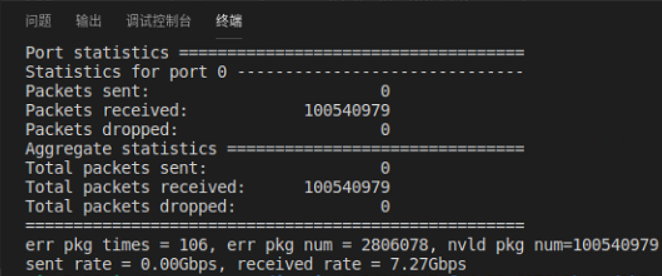
\includegraphics[width = .8\textwidth]{res2.png}
	\caption{乒乓结构下的数据采集结果}
\end{figure}
\begin{figure}[H]
	\centering
	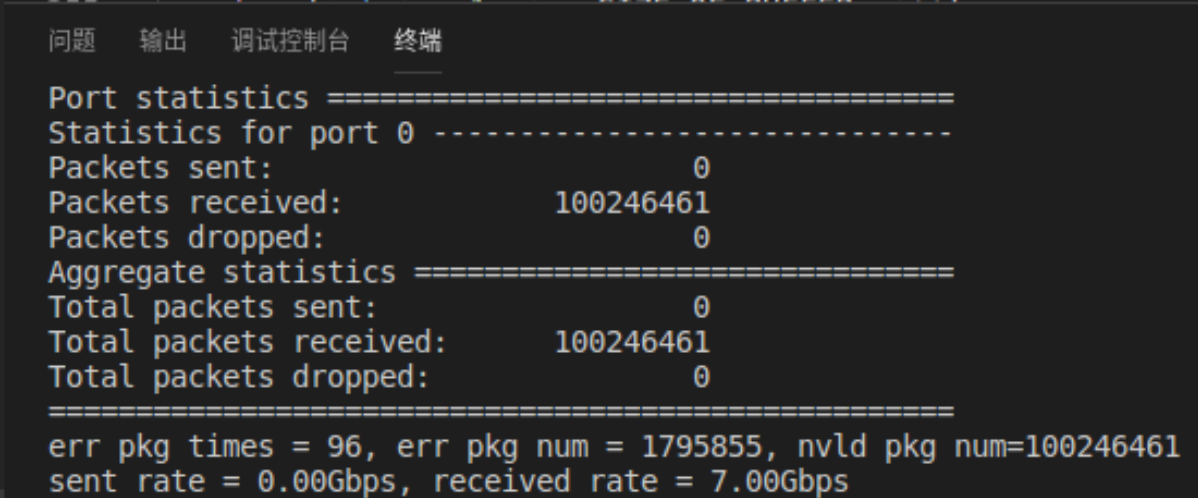
\includegraphics[width = .8\textwidth]{res2f.png}
	\caption{乒乓结构下的数据采集结果(服务器先开)}
\end{figure}
\subsection{乒乓结构}
\begin{figure}[H]
	\centering
	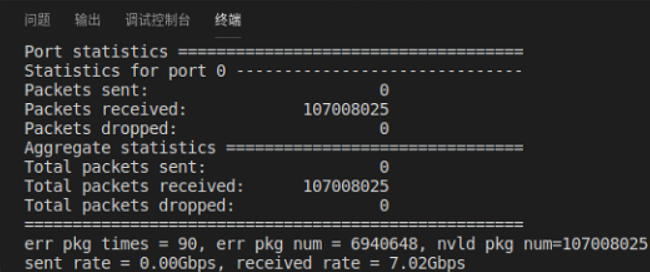
\includegraphics[width = .8\textwidth]{res10.png}
	\caption{N=10的FIFO结构下的数据采集结果}
\end{figure}
\begin{figure}[H]
	\centering
	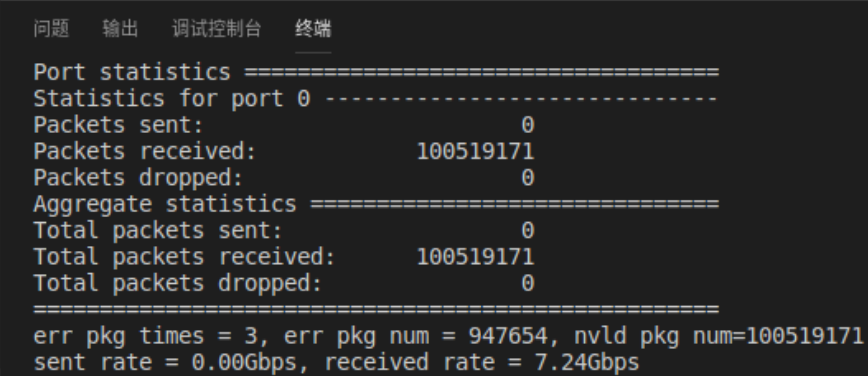
\includegraphics[width = .8\textwidth]{res10f.png}
	\caption{N=10的FIFO结构下的数据采集结果(服务器先开)}
\end{figure}
\begin{figure}[H]
	\centering
	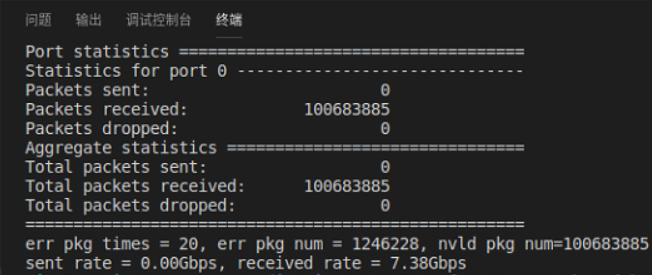
\includegraphics[width = .8\textwidth]{res20.png}
	\caption{N=20的FIFO结构下的数据采集结果}
\end{figure}
\begin{figure}[H]
	\centering
	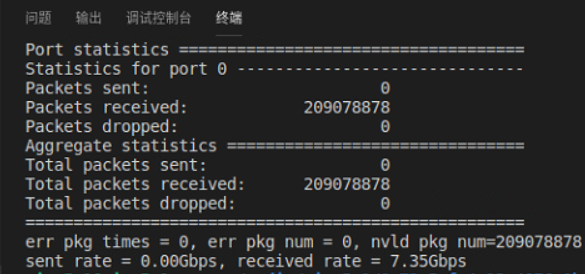
\includegraphics[width = .8\textwidth]{res20f.png}
	\caption{N=20的FIFO结构下的数据采集结果(服务器先开)}
\end{figure}
\subsection{当前问题}
\begin{figure}[H]
	\centering
	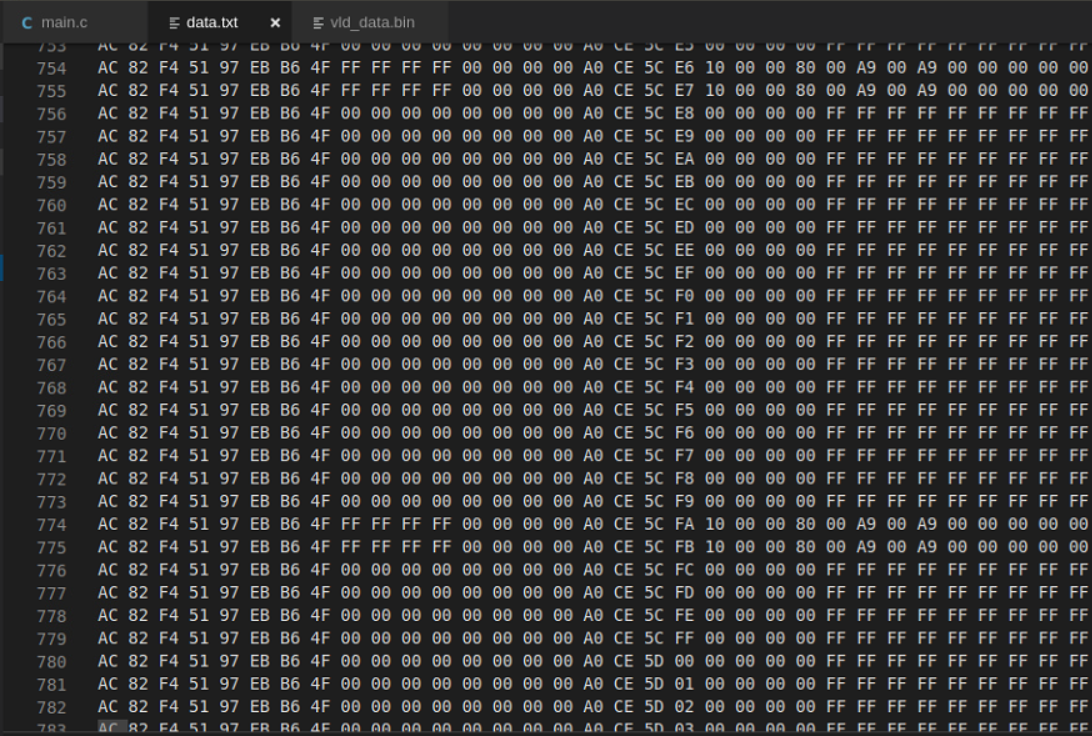
\includegraphics[width = .8\textwidth]{all.png}
	\caption{全部数据}
\end{figure}
\begin{figure}[H]
	\centering
	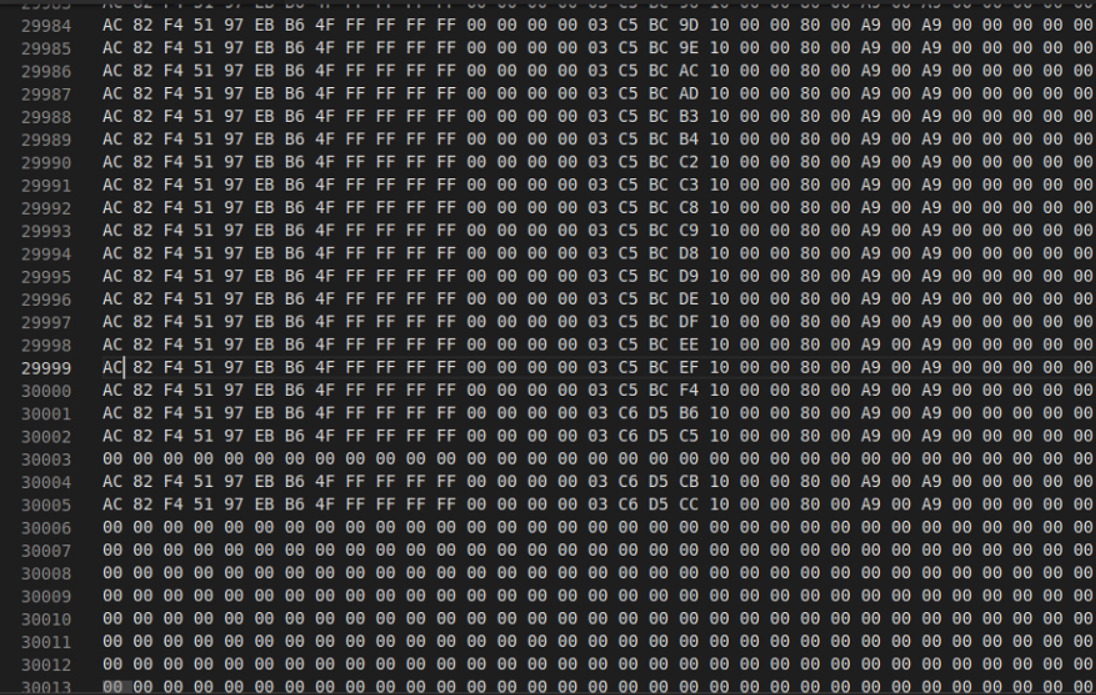
\includegraphics[width = .8\textwidth]{vld.png}
	\caption{有效数据}
\end{figure}
\begin{figure}[H]
	\centering
	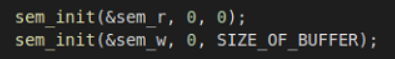
\includegraphics[width = .4\textwidth]{init.png}
	\caption{初始化}
\end{figure}
\begin{figure}[H]
	\centering
	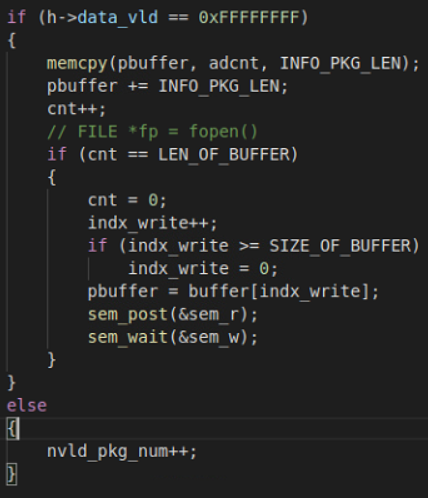
\includegraphics[width = .4\textwidth]{write.png}
	\caption{写}
\end{figure}
\begin{figure}[H]
	\centering
	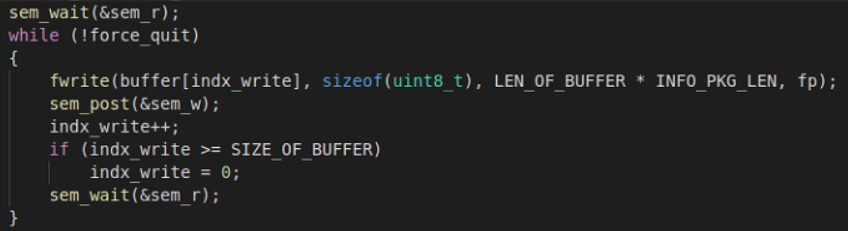
\includegraphics[width = .6\textwidth]{read.png}
	\caption{读}
\end{figure}

%===========第三节=================
\section{完成仿真报告}

%===========第四节=================
% \section{仍存在的问题}


%===========下周计划=================
% \section{下阶段计划}
% 1. 继续完成仿真报告

\end{document}
%%%%%%%%%%%%%%%%%%%%%%%这是正文部分的结束%%%%%%%%%%%%